%GNUPLOT: LaTeX picture with Postscript
\begin{picture}(0,0)%
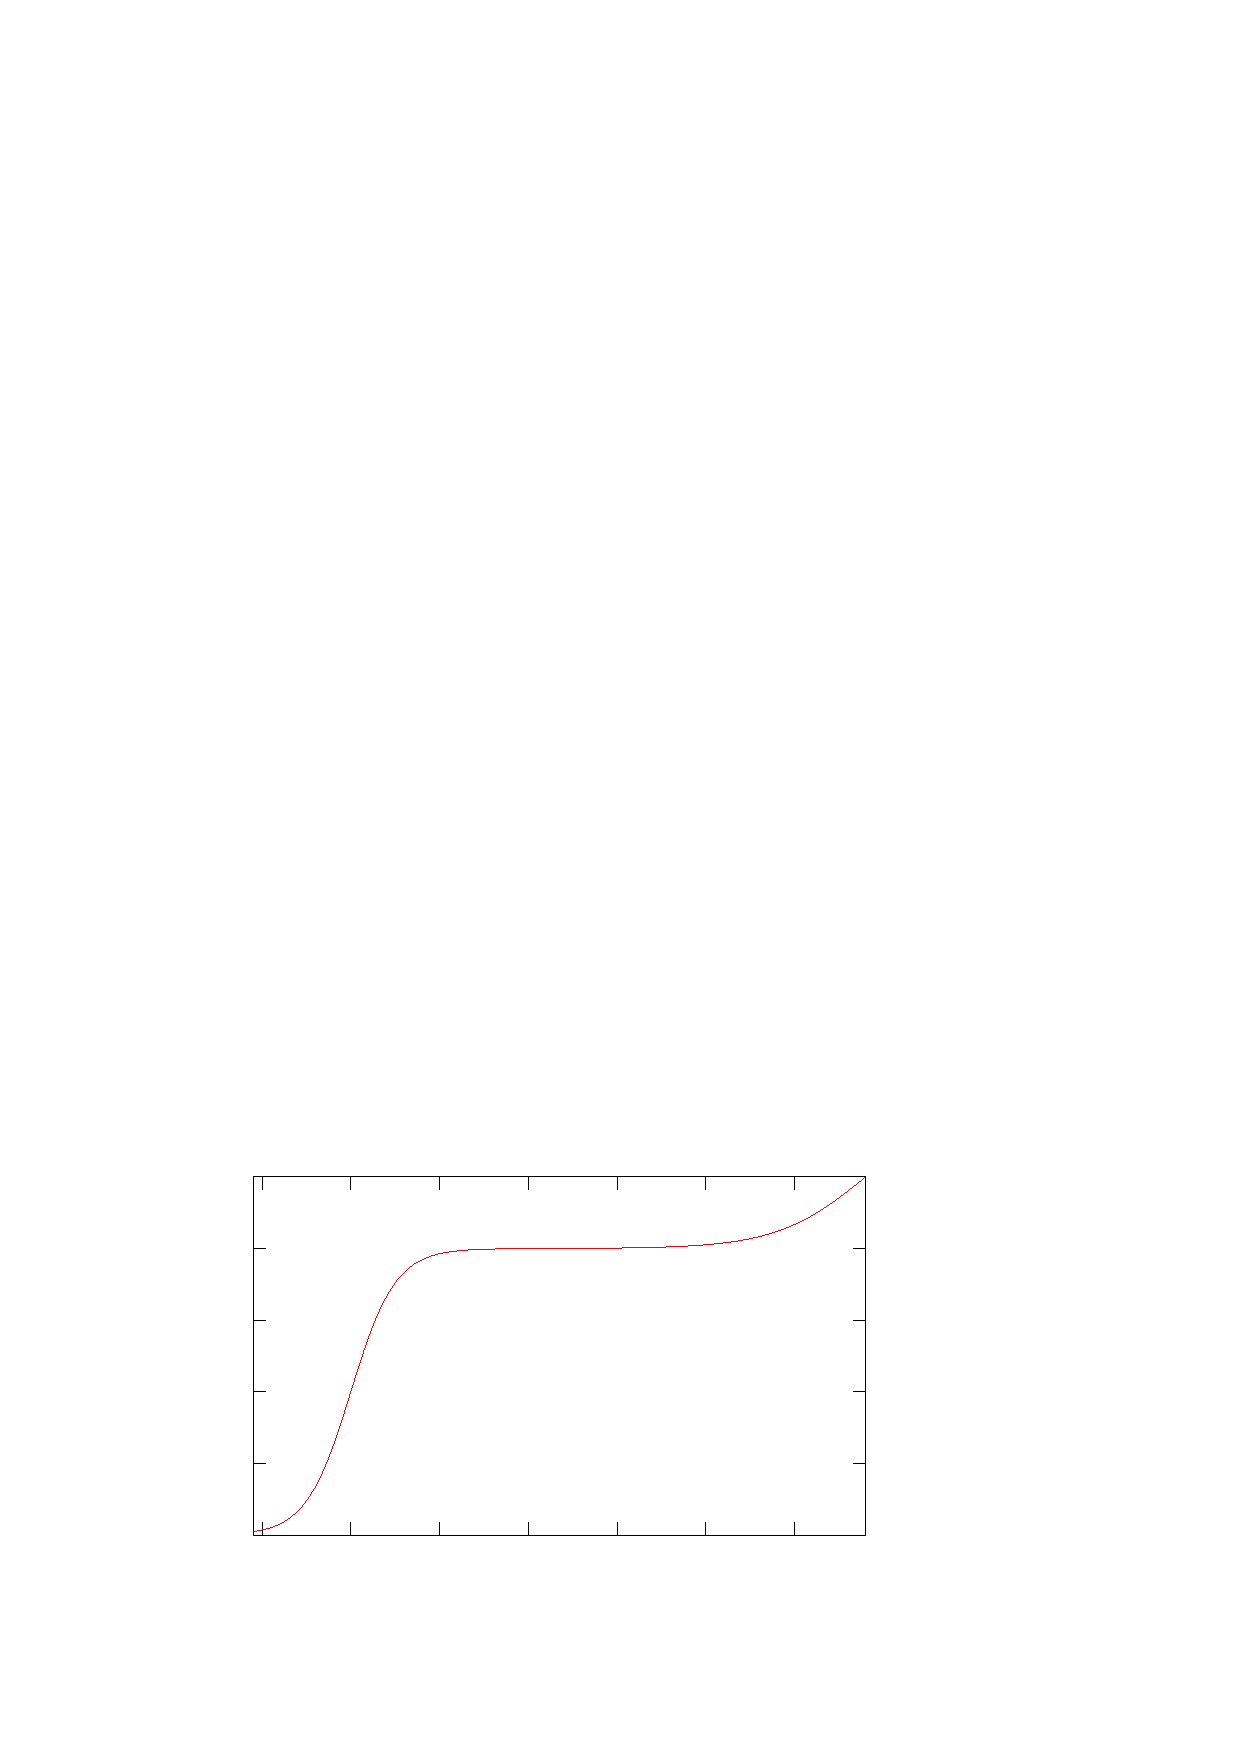
\includegraphics{Graphiques/strato1}%
\end{picture}%
\begingroup
\setlength{\unitlength}{0.0200bp}%
\begin{picture}(18000,10800)(0,0)%
\put(2200,1650){\makebox(0,0)[r]{\strut{}-1.5}}%
\put(2200,3370){\makebox(0,0)[r]{\strut{}-1}}%
\put(2200,5090){\makebox(0,0)[r]{\strut{}-0.5}}%
\put(2200,6810){\makebox(0,0)[r]{\strut{} 0}}%
\put(2200,8530){\makebox(0,0)[r]{\strut{} 0.5}}%
\put(2200,10250){\makebox(0,0)[r]{\strut{} 1}}%
\put(2688,1100){\makebox(0,0){\strut{}-2}}%
\put(4818,1100){\makebox(0,0){\strut{} 0}}%
\put(6949,1100){\makebox(0,0){\strut{} 2}}%
\put(9079,1100){\makebox(0,0){\strut{} 4}}%
\put(11210,1100){\makebox(0,0){\strut{} 6}}%
\put(13340,1100){\makebox(0,0){\strut{} 8}}%
\put(15471,1100){\makebox(0,0){\strut{} 10}}%
\put(550,5950){\rotatebox{90}{\makebox(0,0){\strut{}$f(x; \nombre{11,6})$}}}%
\put(9825,275){\makebox(0,0){\strut{}$x$}}%
\end{picture}%
\endgroup
\endinput
